%  This LaTeX template is based on T.J. Hitchman's work which is itself based on Dana Ernst's template.  
% 
% --------------------------------------------------------------
% Skip this stuff, and head down to where it says "Start here"
% --------------------------------------------------------------
 
\documentclass[12pt]{article}
 
\usepackage[margin=1in]{geometry} 
\usepackage{amsmath,amsthm,amssymb}
\usepackage{graphicx}
\graphicspath{ {./image/} }
\usepackage{sectsty}
\usepackage{pythonhighlight}

\sectionfont{\fontsize{18}{18}\selectfont}
\newenvironment{statement}[2][Statement]{\begin{trivlist}
\item[\hskip \labelsep {\bfseries #1}\hskip \labelsep {\bfseries #2.}]}{\end{trivlist}}

\usepackage{float}
\usepackage{fancyhdr}
\usepackage{titlesec}

\titleformat{\title}{\normalfont\large\bfseries}{\thesection}{1em}{}

\begin{document}
 
% --------------------------------------------------------------
%
%                         Start here
%
% --------------------------------------------------------------
 
\title{\LARGE \textbf{Assignment 1} \\[1ex] Estimation Theory}

\author{
    \textbf{Irsh Vijay}\\
    21EC39055\\
}

\date{}
\maketitle

\section{Problem Statement}
\begin{itemize}
\item Line Fitting
\item Polynomial Fitting
\item Comparing Mean and Max Estimators in DC Estimation
\end{itemize}

\section{Code}
\subsection{Helper Functions}
\textbf{Random Variables:}

\begin{figure}[H] 
\centering 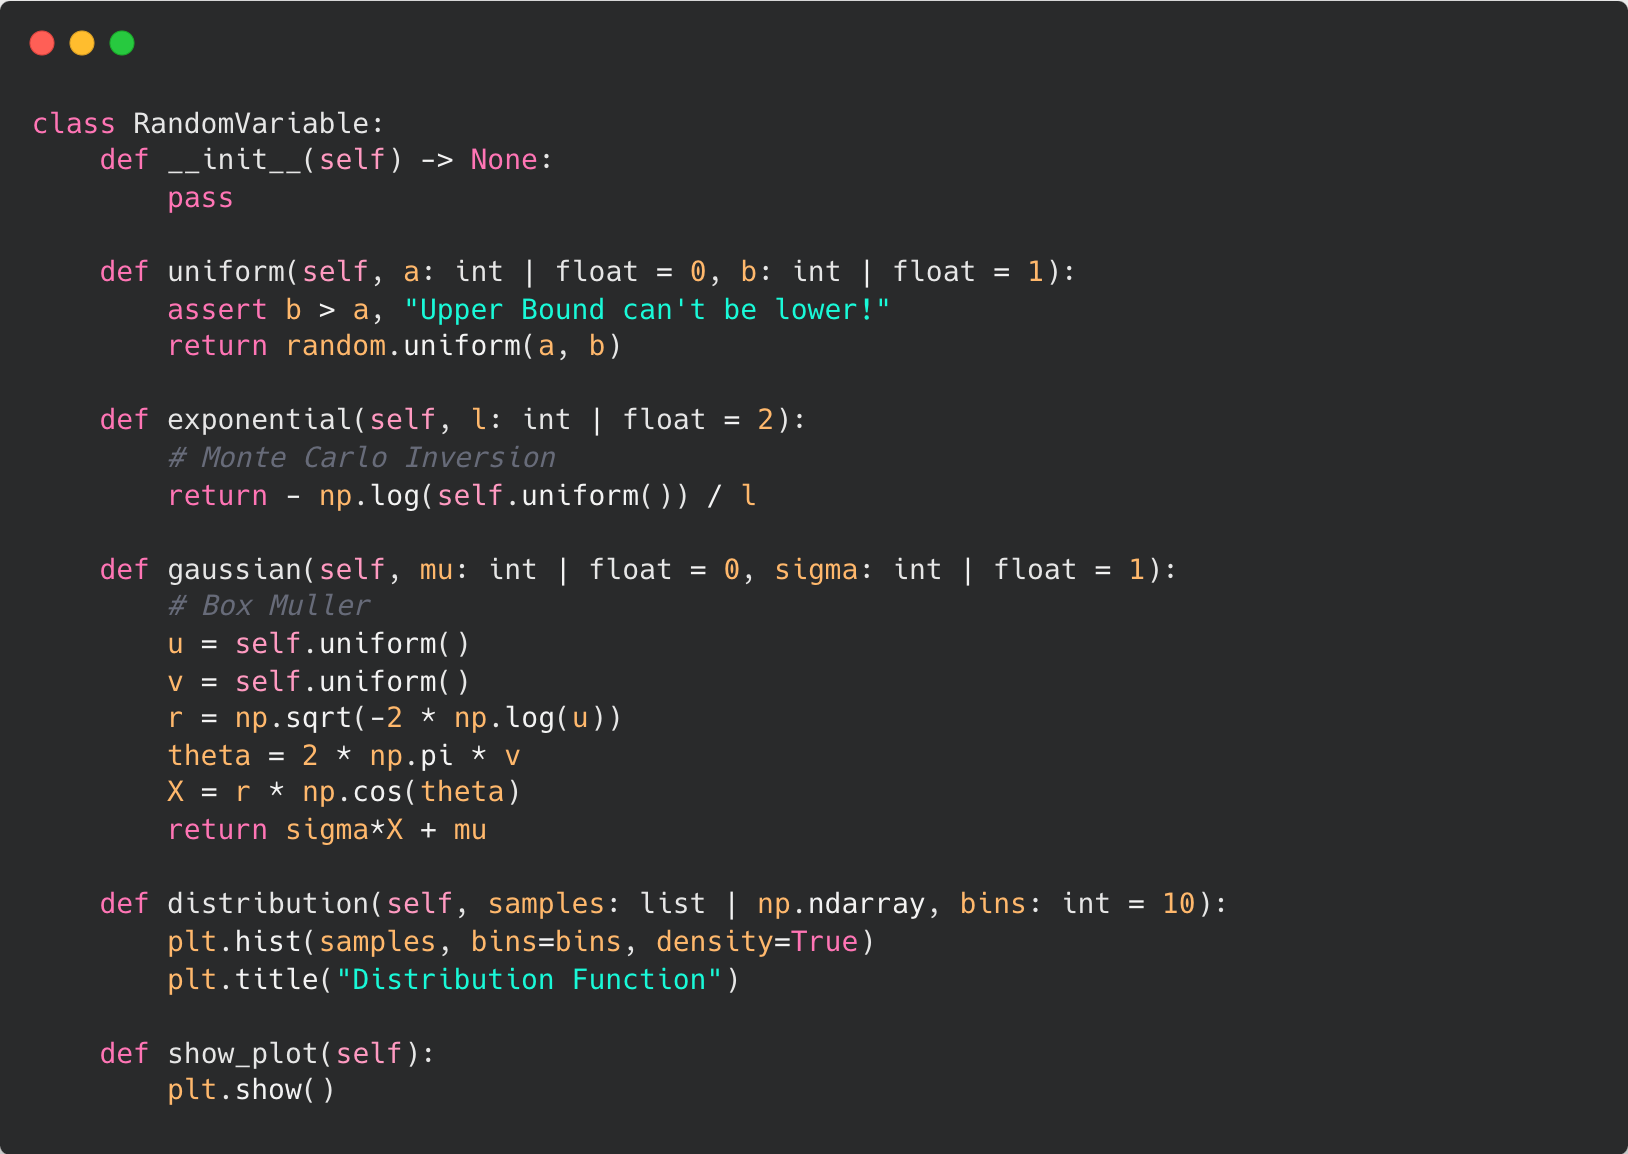
\includegraphics[scale=0.25]{code-rv.png}  
\end{figure}
\raggedright Distributions were generated using Monte Carlo Inversion / Box Muller Transform from a uniform random variable.
\begin{figure}[H] 
\centering 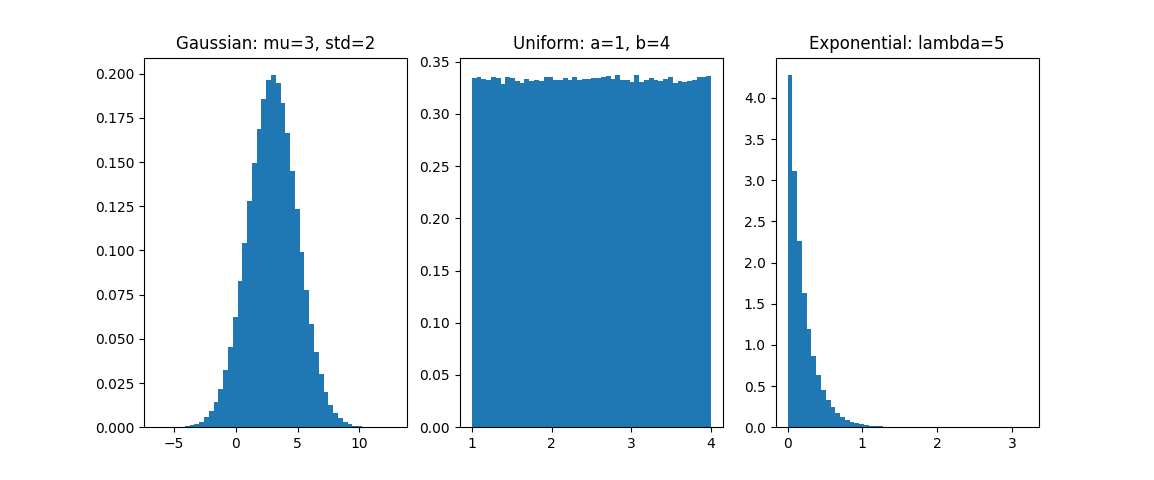
\includegraphics[scale=0.6]{distributions.png}
\end{figure}

\raggedright \textbf{Polynomials:} \newline
Generates polynomial from a list of params (coefficients) and also generates noisy (gaussian) polynomials.
\begin{figure}[H] 
\centering 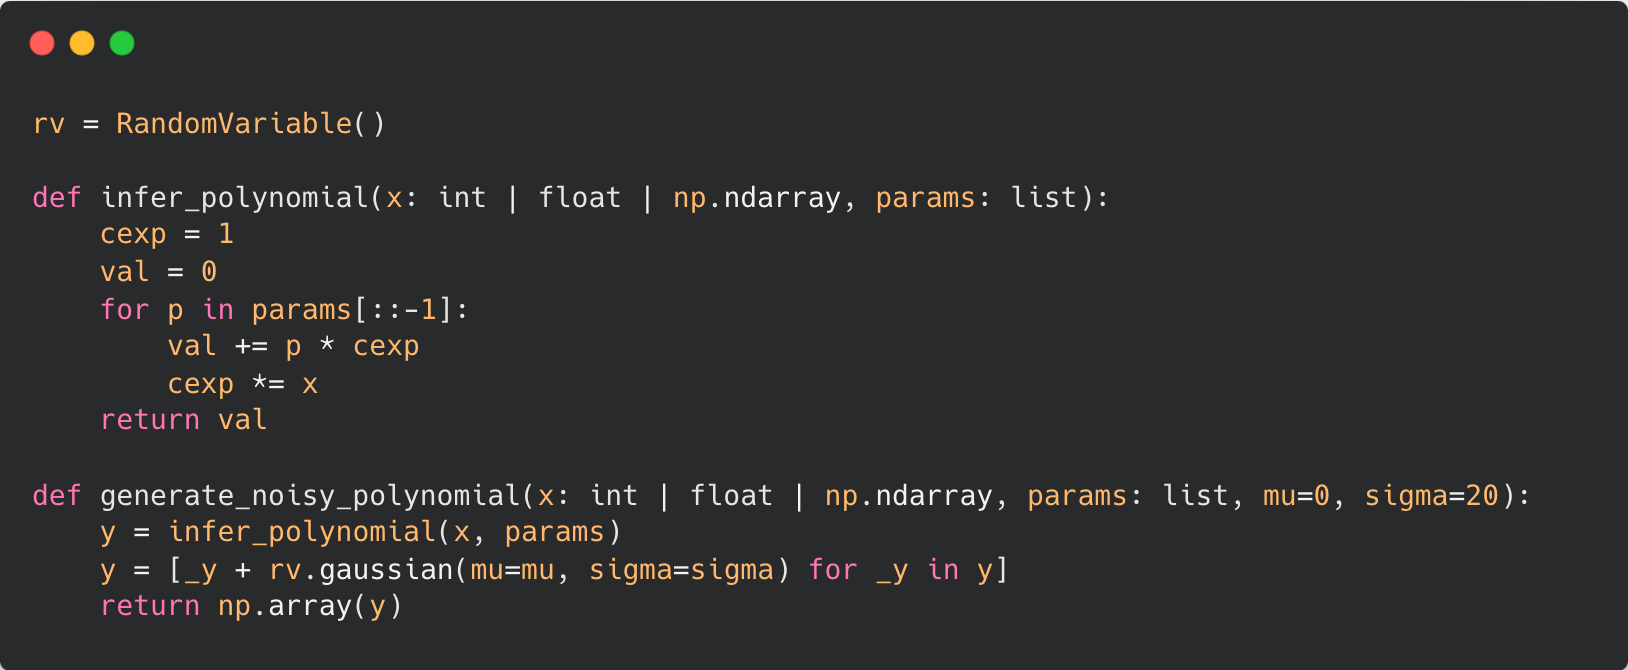
\includegraphics[scale=0.25]{code-poly.png}  
\end{figure}
Plots of few polynomials with noise.
\begin{figure}[H] 
\centering 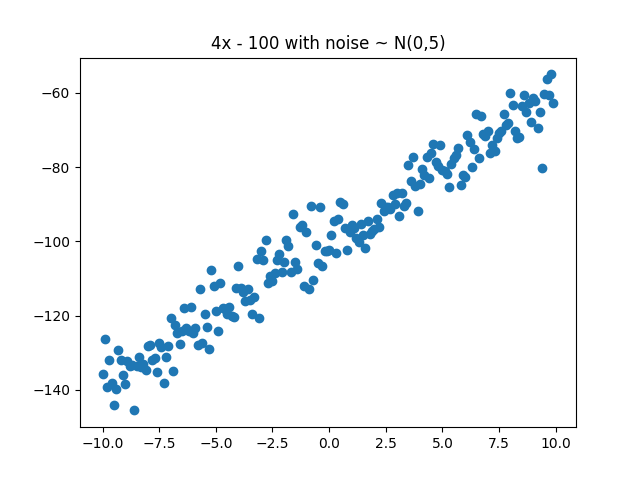
\includegraphics[scale=0.33]{polynomial1.png}
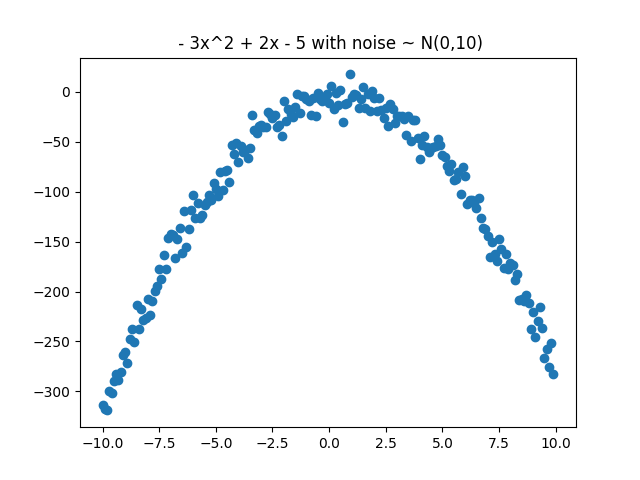
\includegraphics[scale=0.33]{polynomial2.png}
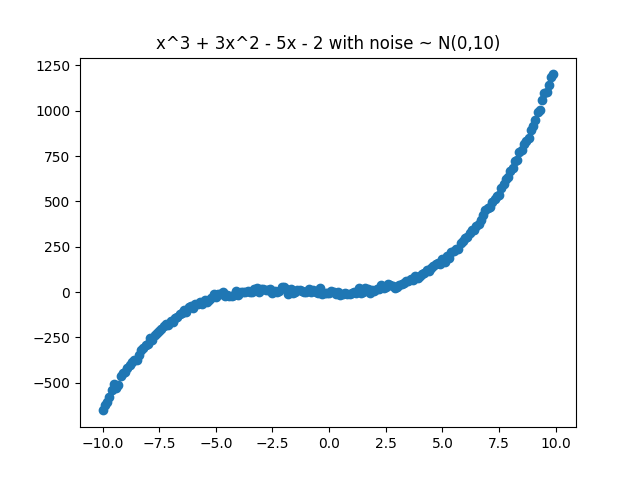
\includegraphics[scale=0.33]{polynomial3.png}
\end{figure}

\raggedright \textbf{Curve Fitting:}
\begin{figure}[H] 
\centering 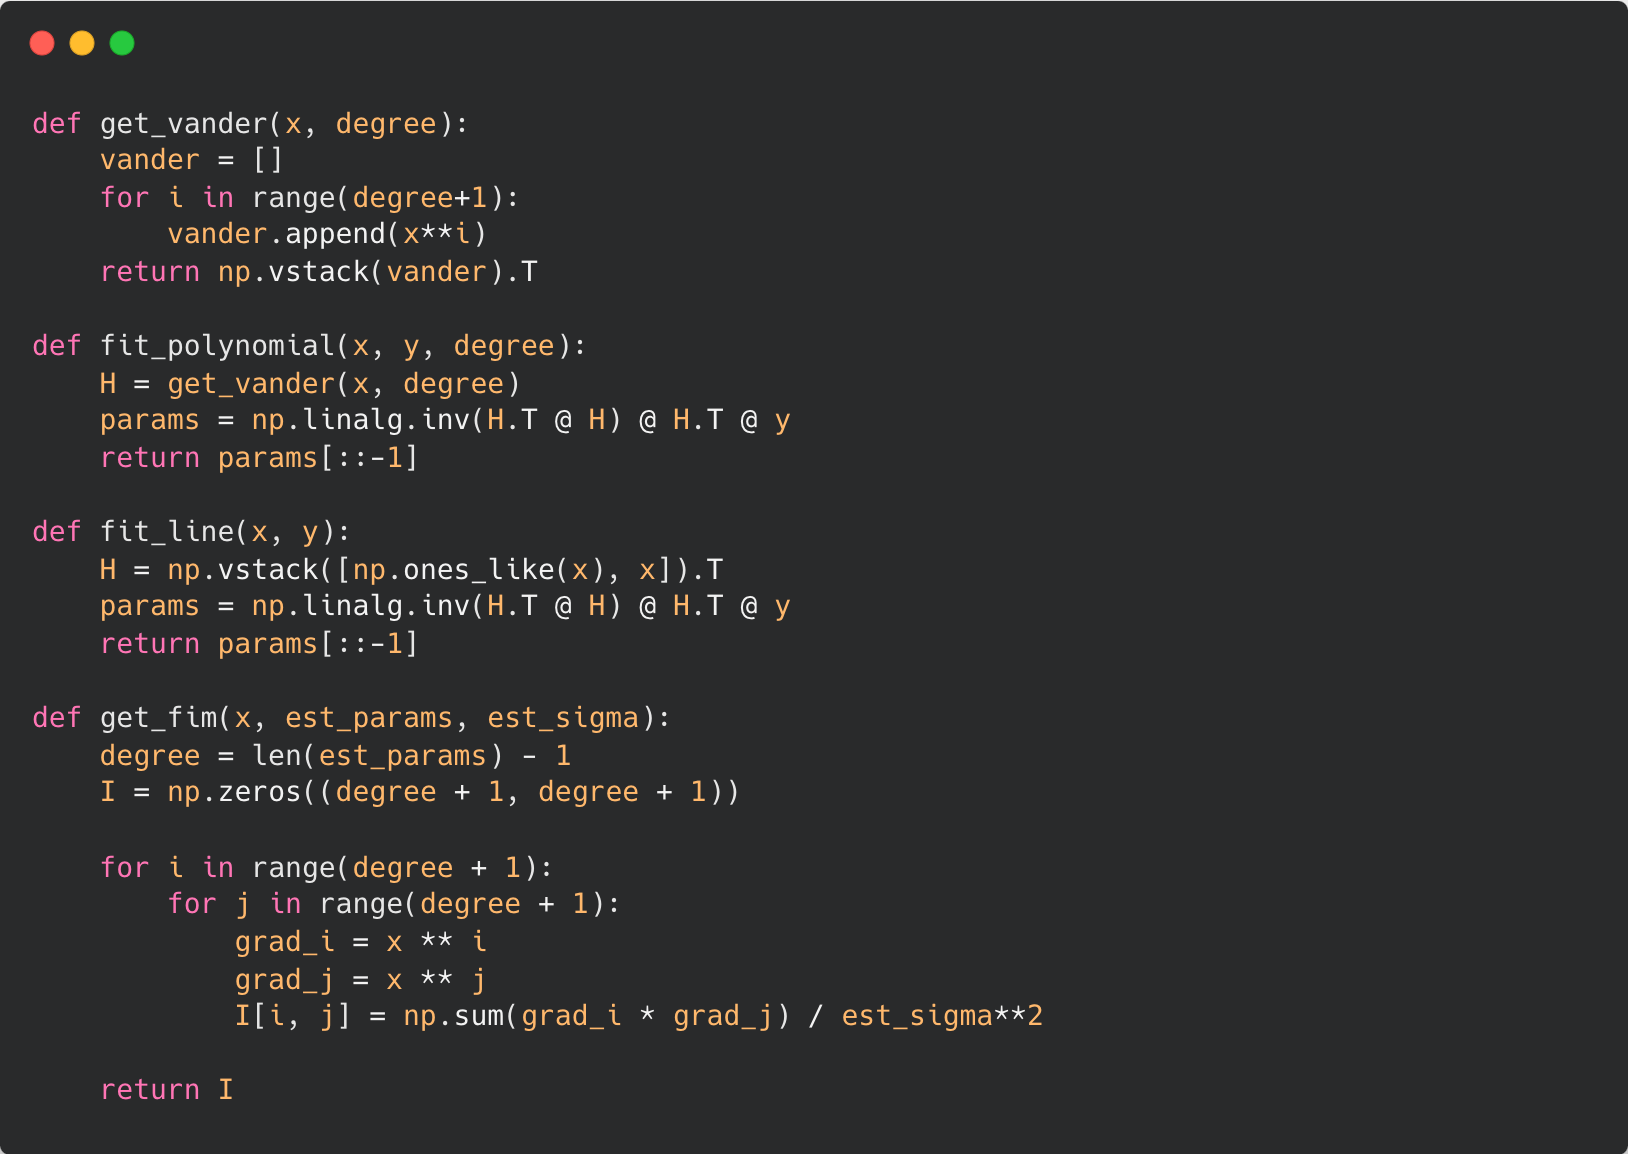
\includegraphics[scale=0.25]{code-curve.png}  
\end{figure}

Contains code for getting the Vandermonde Matrix (get\_vander) and fitting polynomial:

\begin{equation}
    H = \begin{vmatrix}
      1       & x_{0} & x_{0}^{2} & \dots & x_{0}^{n} \\ 
      1       & x_{1} & x_{1}^{2} & \dots & x_{1}^{n} \\
      \vdots  & \vdots&  \vdots   &       & \vdots    \\
      1       & x_{n} & x_{n}^{2} & \dots & x_{n}^{n} \\ 
    \end{vmatrix}
\end{equation}
\newline
\begin{equation}
    \theta = (H^TH)^{-1}H^Ty = H^{\dag}y
\end{equation}

\newpage
\subsection{Main Code}
\textbf{Line Fitting}
\begin{figure}[H] 
\centering 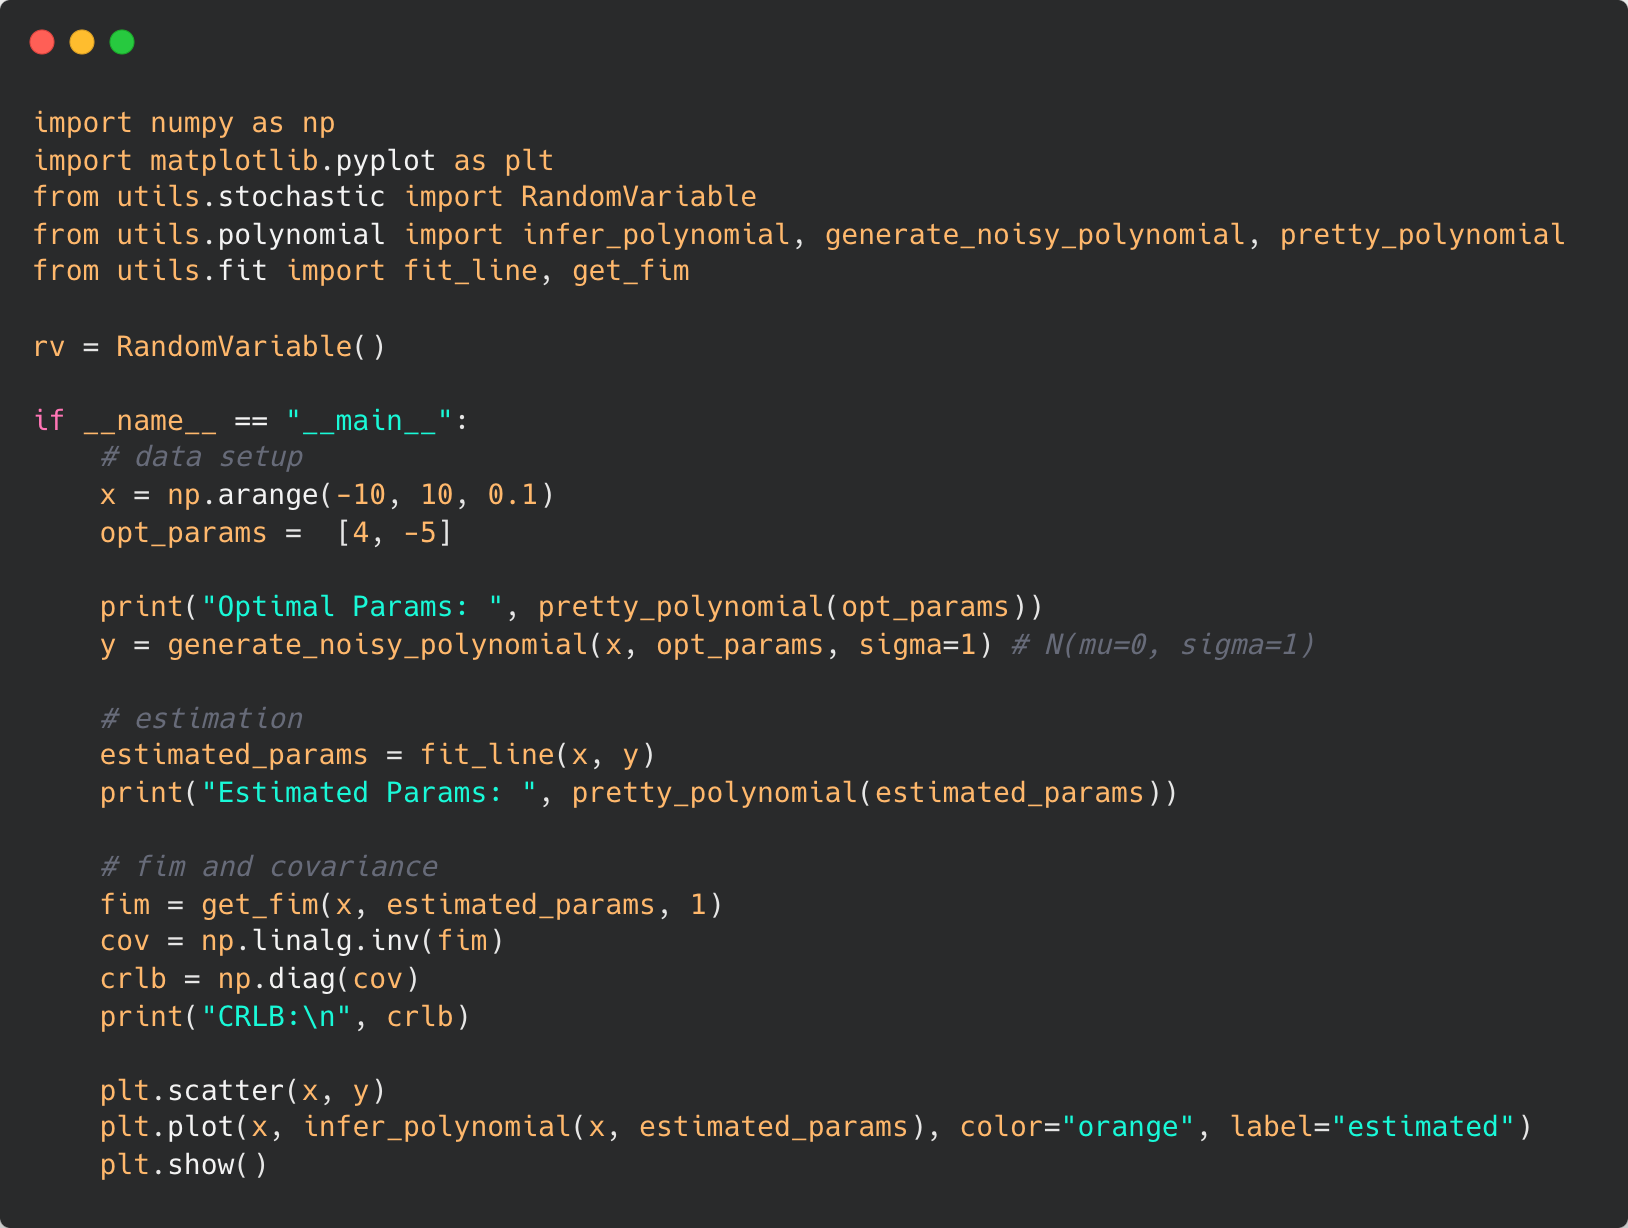
\includegraphics[scale=0.2]{code-lf.png}  
\end{figure}
\textbf{Polynomial Fitting}
\begin{figure}[H] 
\centering 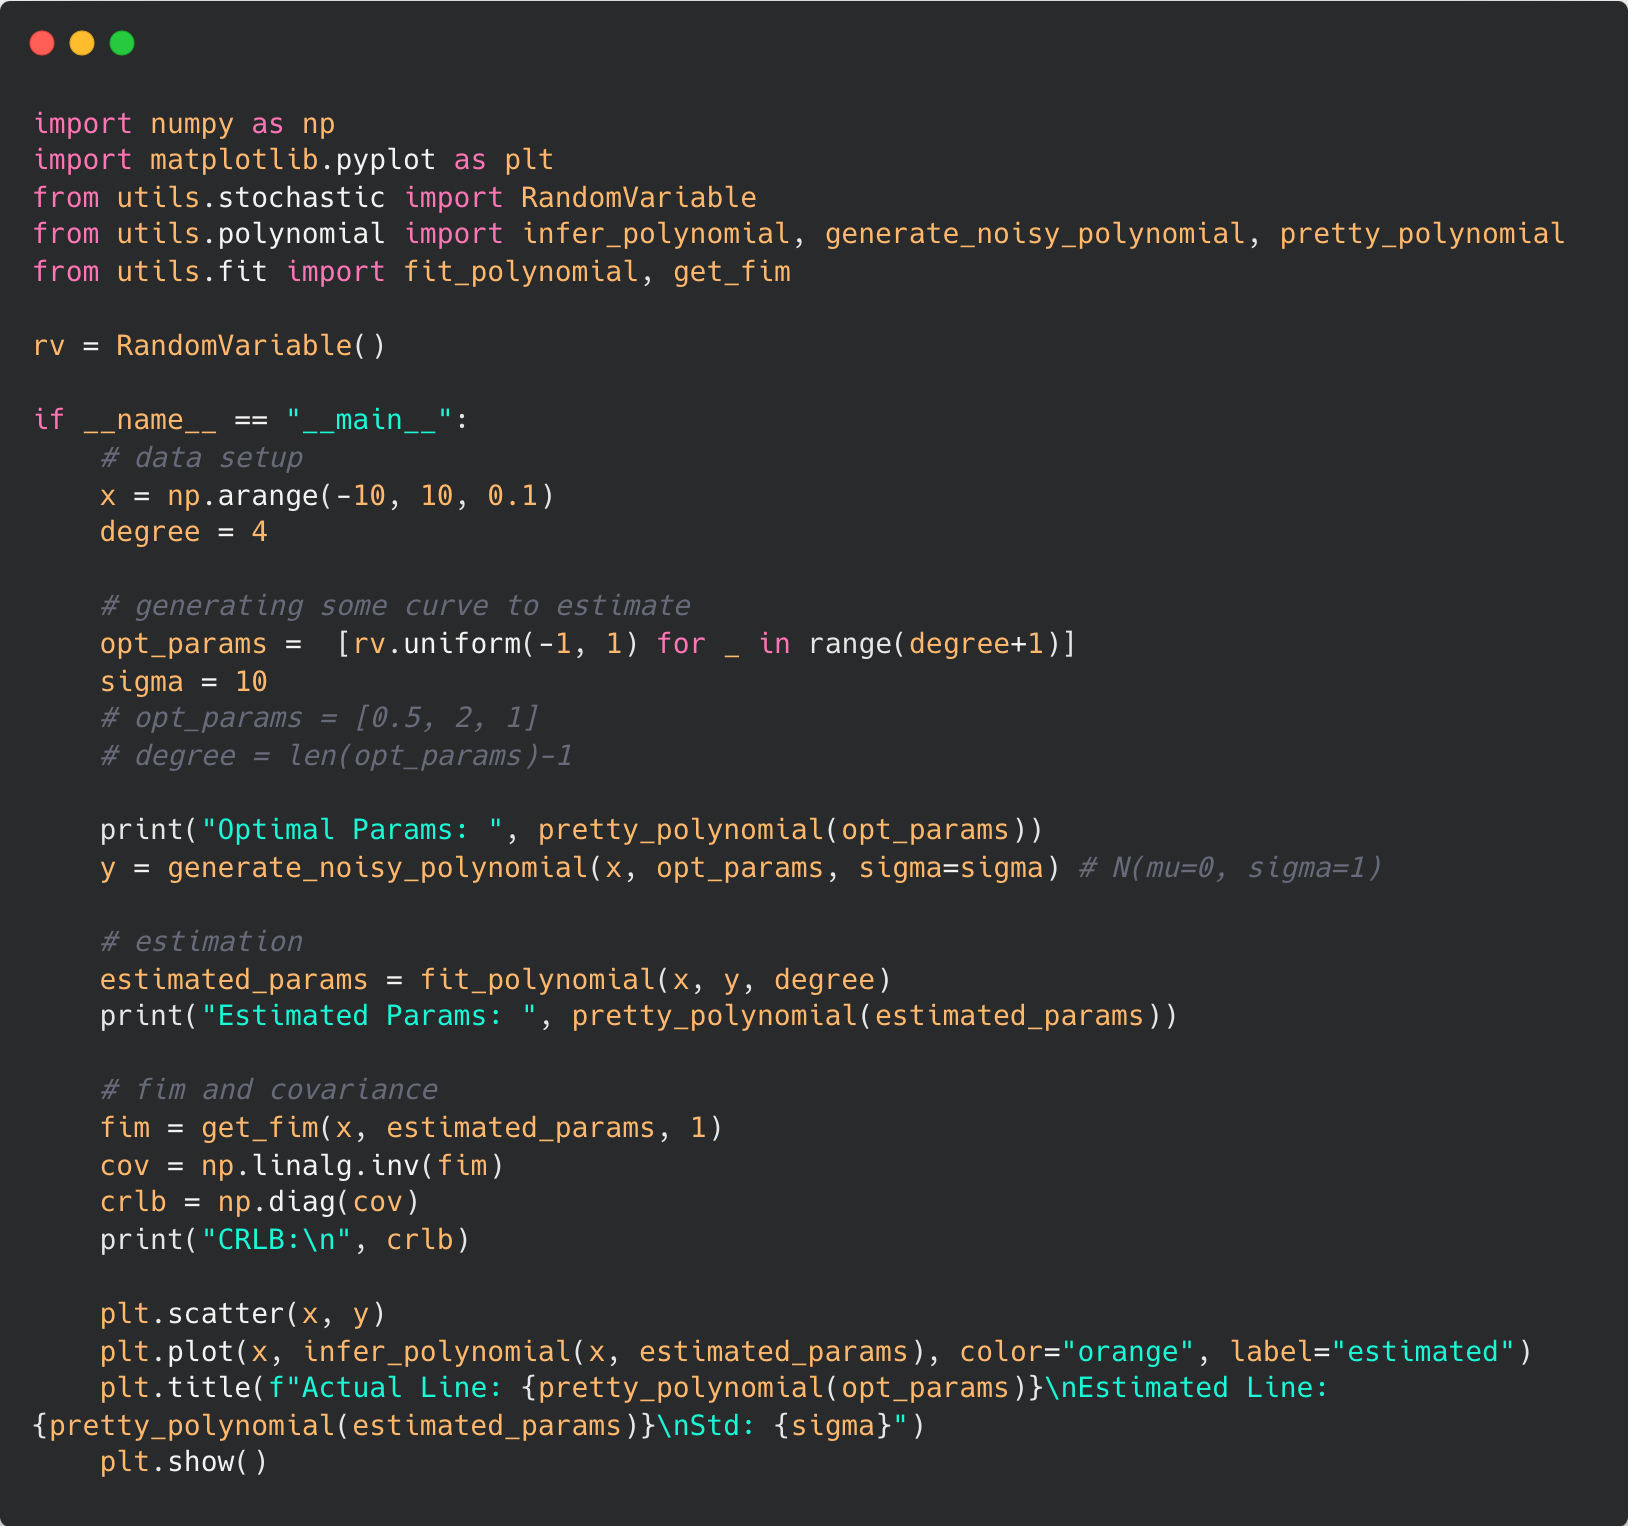
\includegraphics[scale=0.2]{code-pf.png}  
\end{figure}
\textbf{Comparing Mean and Max Estimators}
\begin{figure}[H] 
\centering 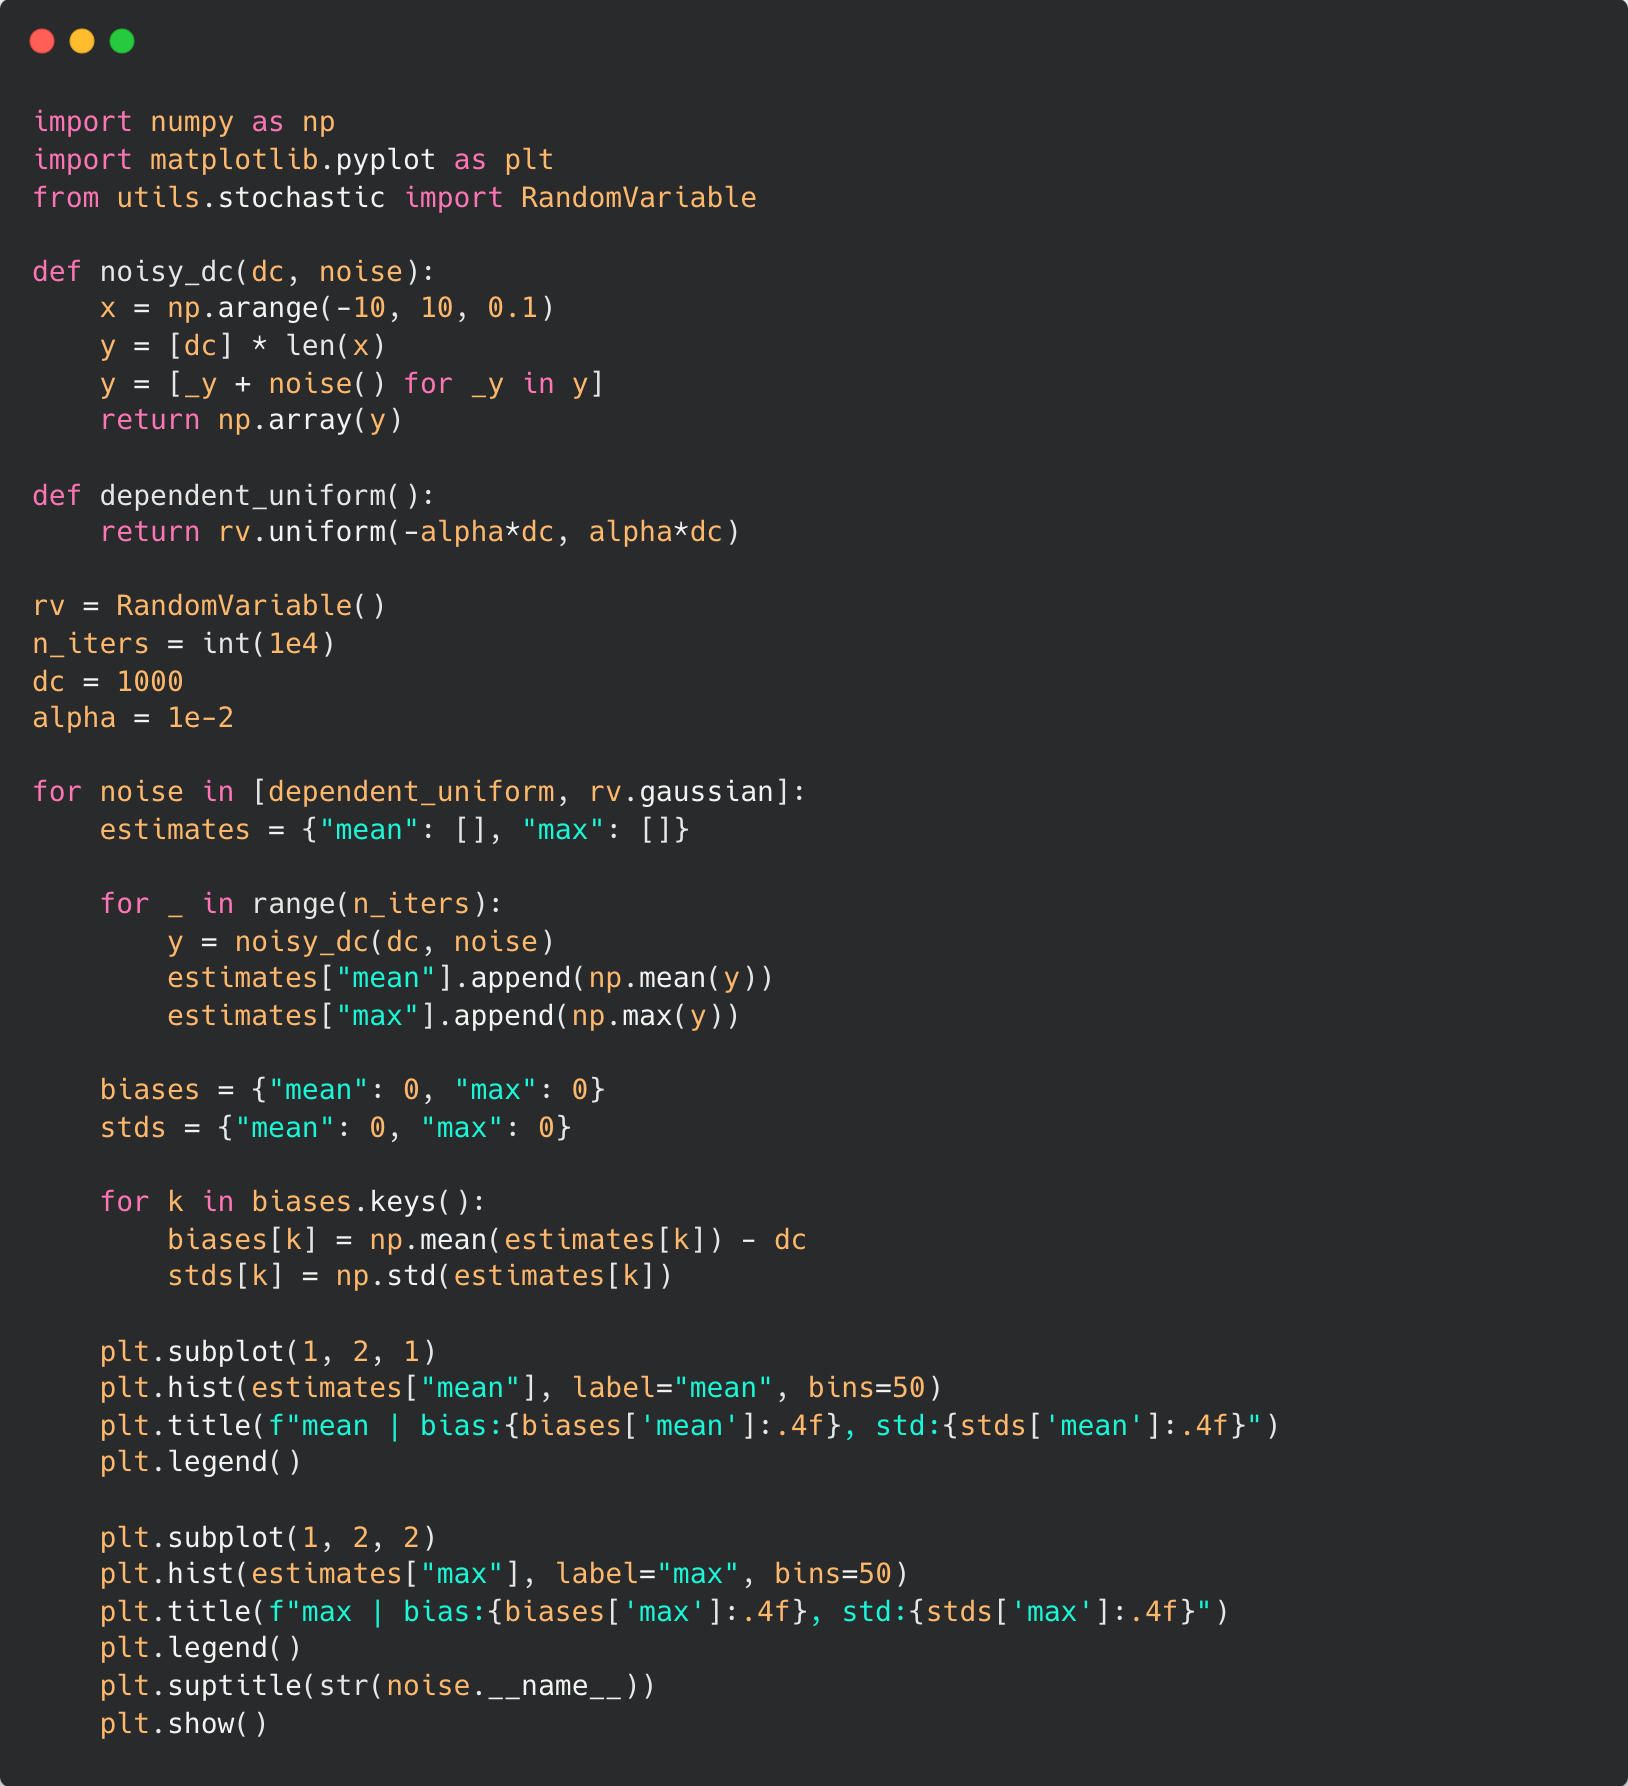
\includegraphics[scale=0.2]{code-ce.png}  
\end{figure}

\section{Results}
\textbf{Line Fitting}
\begin{figure}[H] 
\centering 
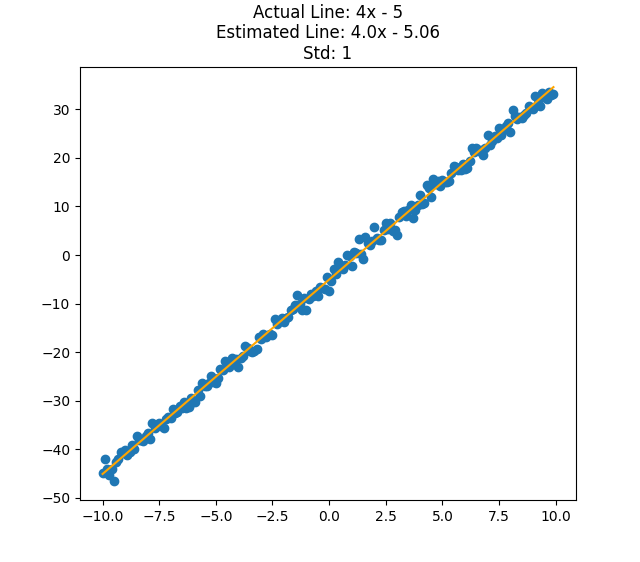
\includegraphics[scale=0.33]{line1.png}
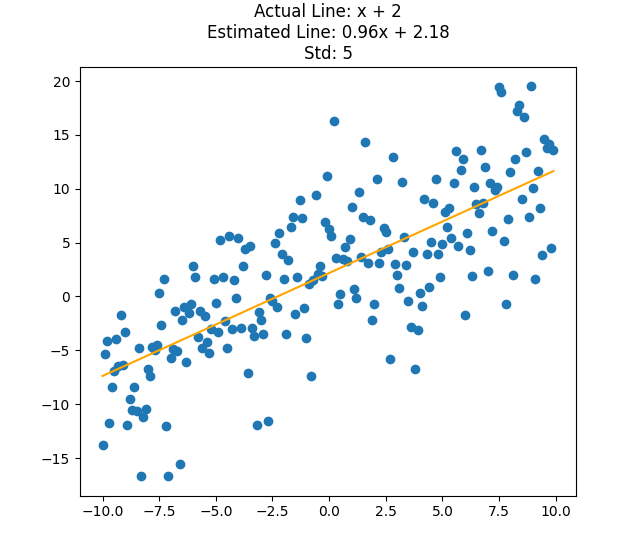
\includegraphics[scale=0.33]{line2.png}  
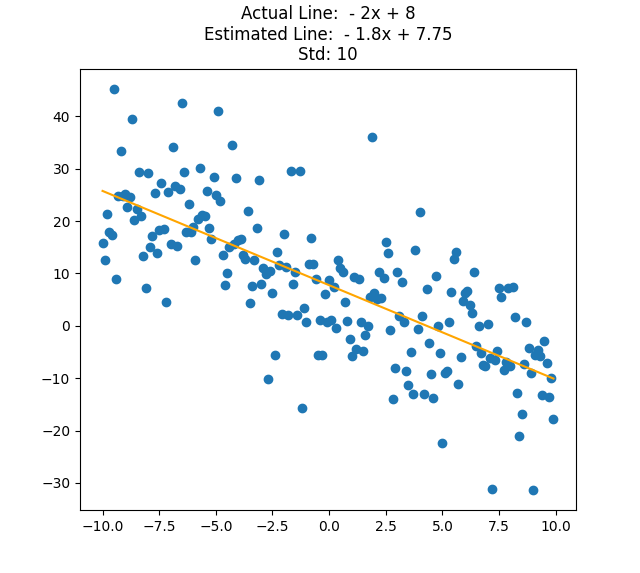
\includegraphics[scale=0.33]{line3.png}  
\end{figure}
\newpage
\textbf{Polynomial Fitting}
\begin{figure}[H] 
\centering 
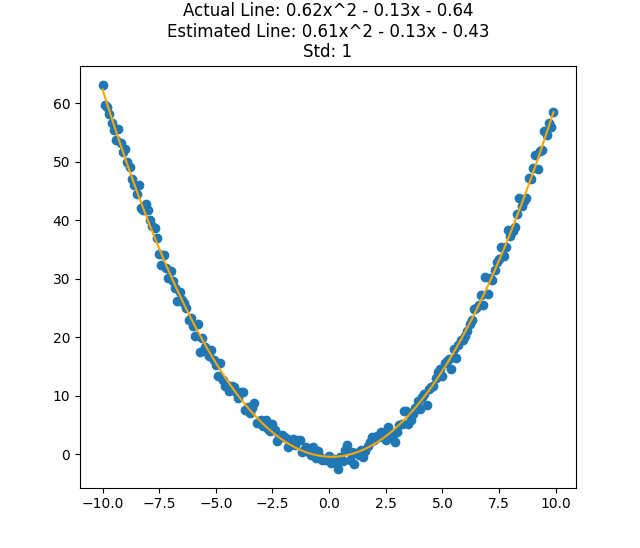
\includegraphics[scale=0.33]{pf1.png}
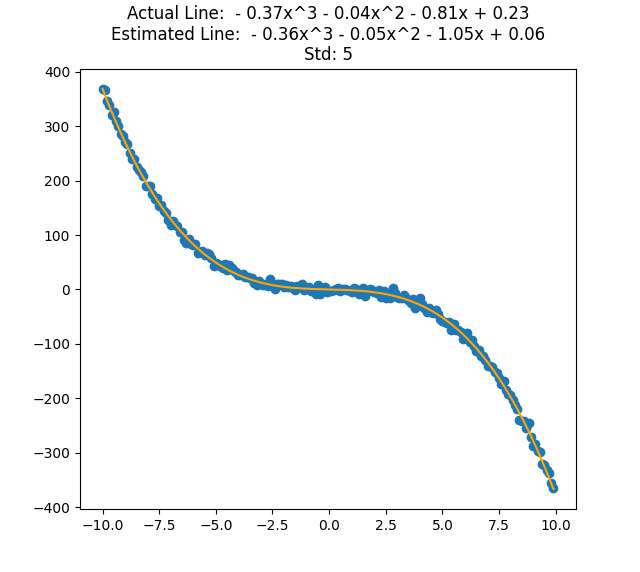
\includegraphics[scale=0.33]{pf2.png}  
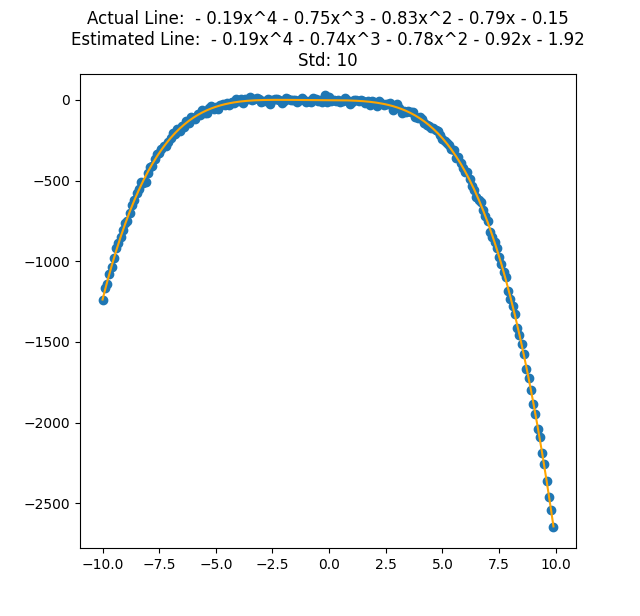
\includegraphics[scale=0.33]{pf3.png}  
\end{figure}
\textbf{Mean vs Max Estimators} \newline
Parameter Dependent Uniform - \math{U(-\alpha*dc,\alpha*dc)}

\begin{figure}[H] 
\centering 
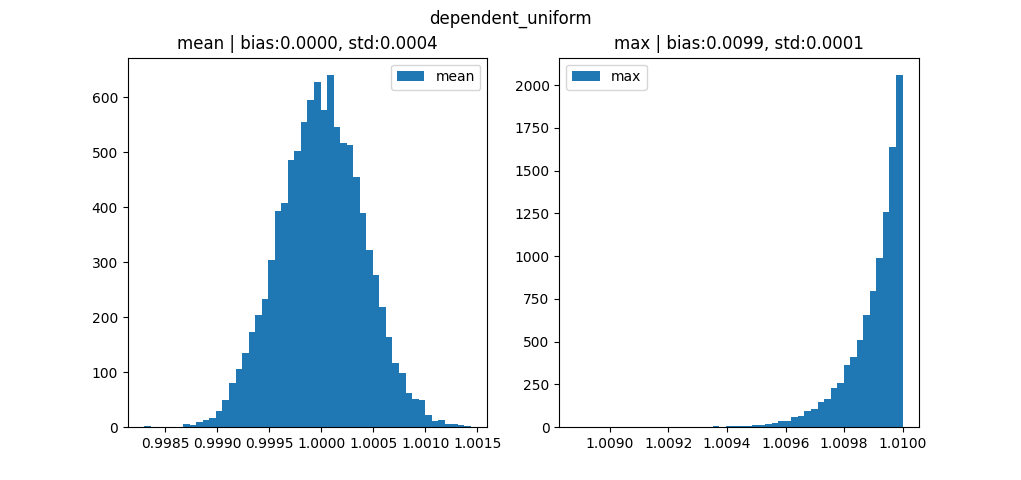
\includegraphics[scale=0.5]{ce-du-low.png}
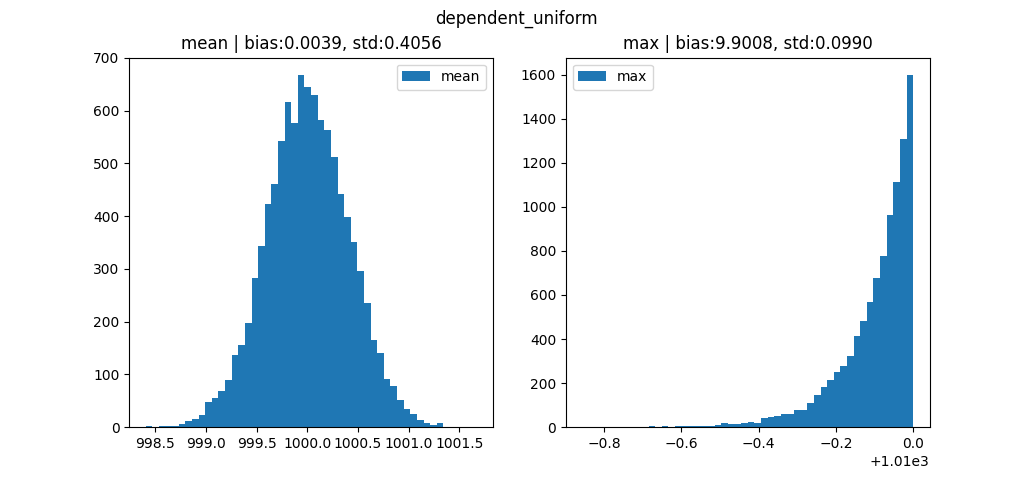
\includegraphics[scale=0.5]{ce-du-hi.png}
\caption{(a) DC=1, (b) DC=1000}
\end{figure}

\newpage
Gaussian - \math{N(0, 1)}

\begin{figure}[H] 
\centering 
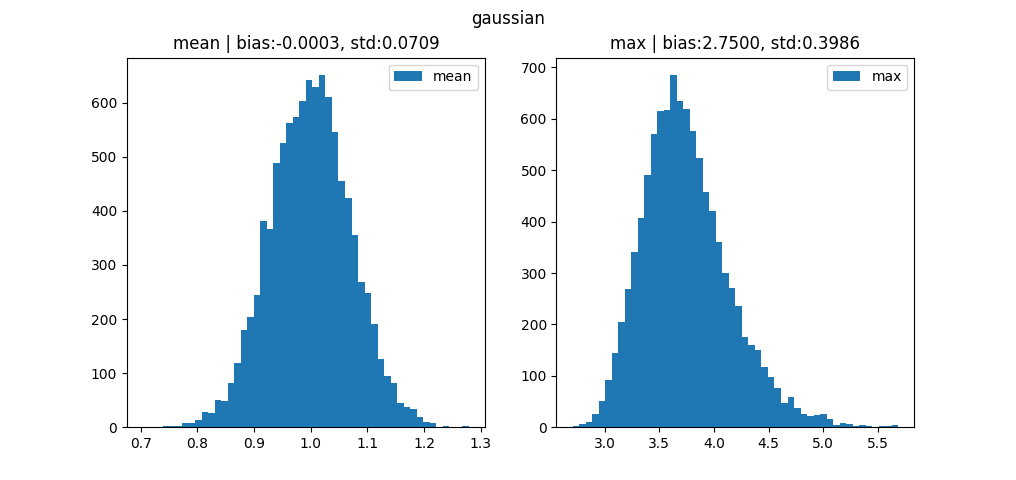
\includegraphics[scale=0.5]{ce-ga-low.png}
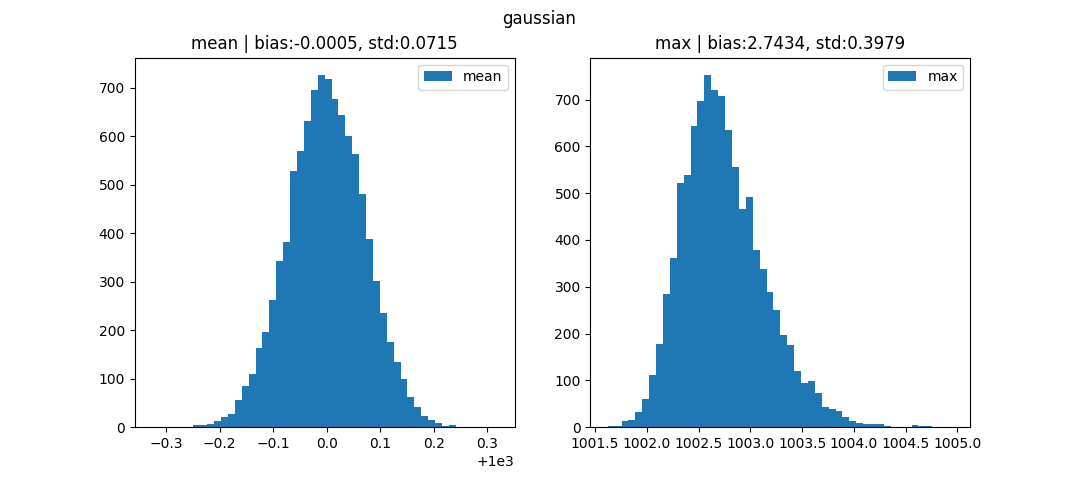
\includegraphics[scale=0.5]{ce-ga-hi.png}
\caption{(a) DC=1, (b) DC=1000}
\end{figure}

\section{Discussion}
\begin{itemize}
    \item I generated different types of random variables and was able to verify Law of Large Numbers when I varied number of samples as it more closely approximated the real distribution.
    \item Using the random variable I had made before I modeled the input data (with gaussian noise)
    \item Then for the first two parts, the equations for polynomial regression were used to get estimations for the polynomial coefficients
    
        \begin{equation*}
            H = \begin{vmatrix}
              1       & x_{0} & x_{0}^{2} & \dots & x_{0}^{n} \\ 
              1       & x_{1} & x_{1}^{2} & \dots & x_{1}^{n} \\
              \vdots  & \vdots&  \vdots   &       & \vdots    \\
              1       & x_{n} & x_{n}^{2} & \dots & x_{n}^{n} \\ 
            \end{vmatrix}
        \end{equation*}
        \newline
        \begin{equation*}
            \theta = (H^TH)^{-1}H^Ty = H^{\dag}y
        \end{equation*}

    \item The polynomial corresponding to the theta value was then plotted and the Fisher Information Matrix and Cramer Rao Lower Bound was calculated.
        \begin{equation*}
            CRLB = I^{-1}(\theta)
        \end{equation*}
    \item For comparing the mean and max estimators, first a "dependent" uniform random variable was created: 
    \begin{equation*}
        U(-\alpha*DC,\alpha*DC), \alpha=0.01
    \end{equation*}
    \item It was interesting to see that for the dependent uniform, the mean estimator followed a bell-like curve and the max estimator was similar to a flipped exponential.
    \item When the DC value was high, the max estimator was more precise in the case of the gaussian.
    
        
        

\end{itemize}



% --------------------------------------------------------------
%     You don't have to mess with anything below this line.
% --------------------------------------------------------------
 
\end{document}